Nous allons proposer une définition simple de la convexité pour les \ngones, et plus généralement pour les \ncycles. Ceci demande de savoir que, dans un plan orienté, le triangle non dégénéré $ABC$ est dit \focus{orienté positivement} si la condition $\det \big( \vect{AB} , \vect{AC} \big) > 0$ est validée (dans ce cas, le triangle $BAC$ est orienté négativement, comme on le vérifie facilement).
Pourquoi étudier la convexité des \ncycles? Pour l'existence d'au moins un solution, nous travaillerons dans un ensemble compact, et donc fermé, de \ncycles, or, pour garder des \ngones, nous devrions utiliser des non-égalités, mais ceci nous ferait sortir du cadre fermé qui nous intéresse.


% ----------------------- %


\begin{defi} \label{conv-ncycle-def}
	Un \ncycle\ $\setproba{L} = A_1 A_2 \cdots A_n$ est dit \focus{convexe} si  l'une des alternatives suivantes a lieu.
    %
	\begin{itemize}
		\item $\forall (i, k) \in \ZintervalC{1}{n}^2$,
		$\det \big( \vect{\primeit{A}_i \primeit{A}_{i+1}}, \vect{\primeit{A}_i \primeit{A}_k} \big) \geq 0$.

		\item $\forall (i, k) \in \ZintervalC{1}{n}^2$,
		$\det \big( \vect{\primeit{A}_i \primeit{A}_{i+1}}, \vect{\primeit{A}_i \primeit{A}_k} \big) \leq 0$.
    \end{itemize}
	
	Autrement dit, $\setproba{L} = A_1 A_2 \cdots A_n$ est convexe si l'une des alternatives suivantes a lieu.
    %
	\begin{itemize}
		\item $\forall (i, k) \in \ZintervalC{1}{n}^2$,
		$\primeit{A}_i \primeit{A}_{i+1} \primeit{A}_k$ est soit dégénéré, soit  orienté positivement.

		\item $\forall (i, k) \in \ZintervalC{1}{n}^2$,
		$\primeit{A}_i \primeit{A}_{i+1} \primeit{A}_k$ est soit dégénéré, soit  orienté négativement.
    \end{itemize}
\end{defi}


\begin{remark}
    Voici des exemples pour clarifier le vocabulaire.	
    
    \begin{center}
    	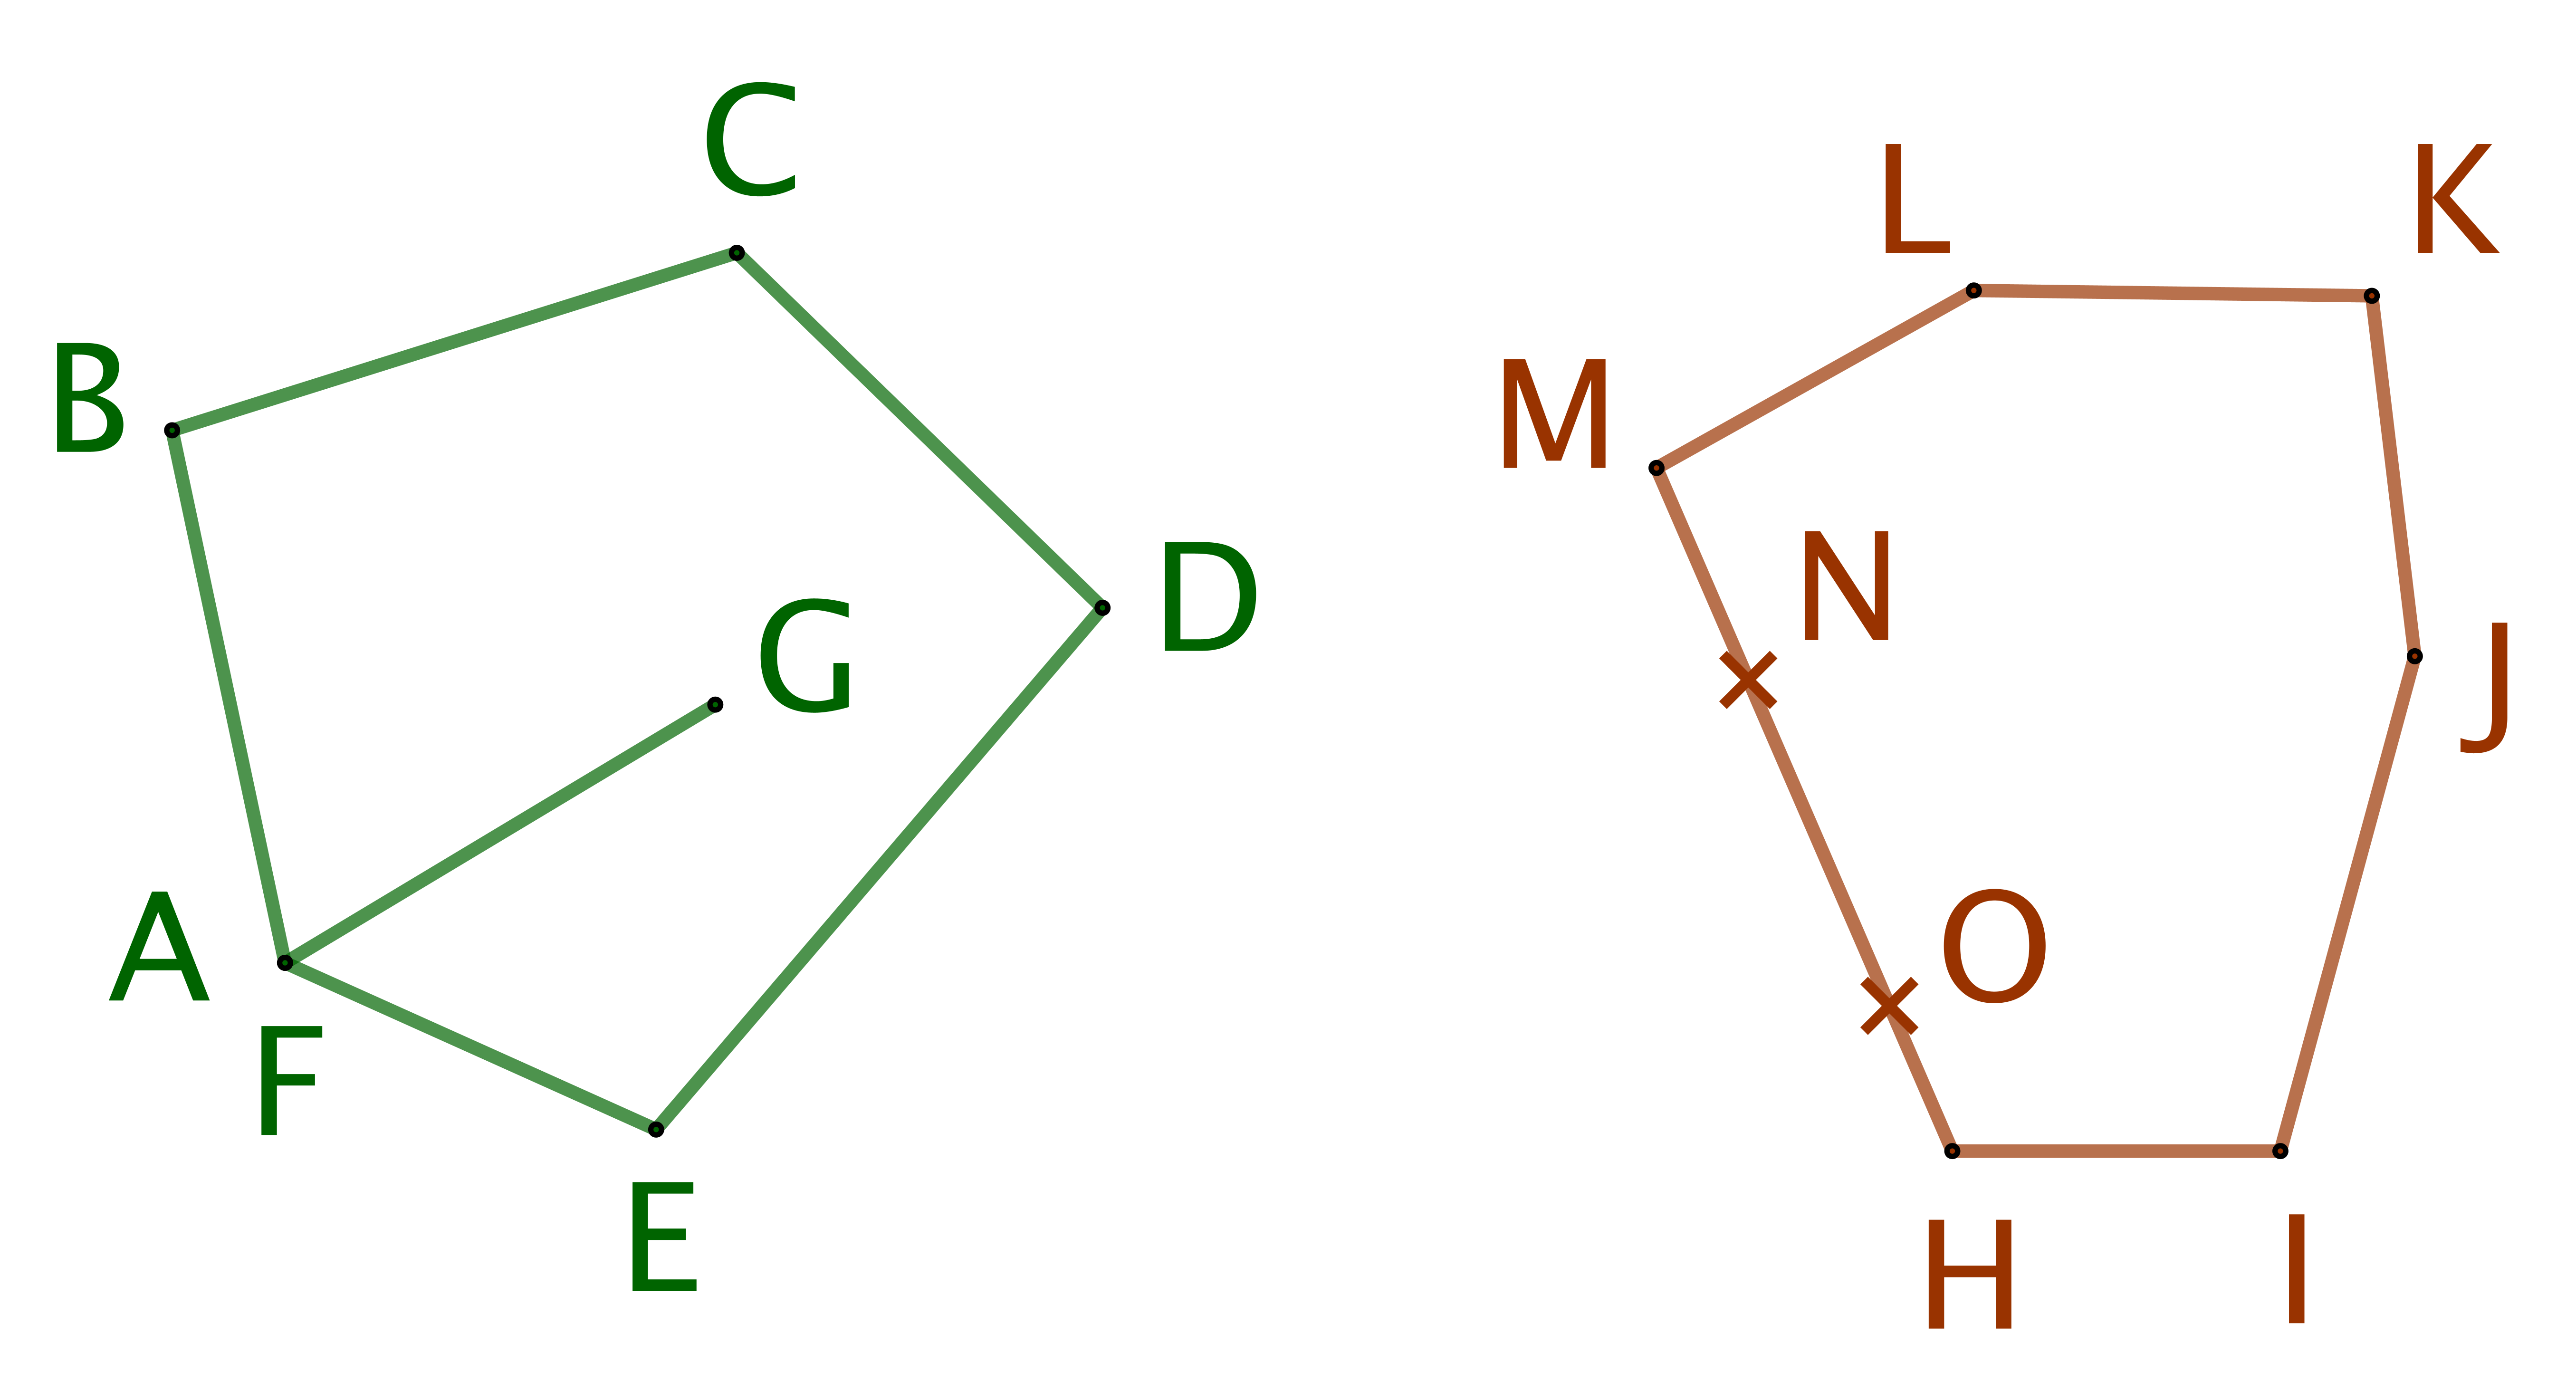
\includegraphics[scale=.3]{content/polygon/convex/degenerated-ncycles.png}
    \end{center}
    
    Le \xcycle{7} non dégénéré $ABCDEFG$ n'est pas convexe, à cause, par exemple, des triangles d'orientations opposées $FGE$ et $FGC$.%
    \footnote{
        $ABCDEFG$ n'est pas un \xgone{7}, car les trois sommets consécutifs $F$, $G$ et $A$ sont alignés.
    }
    Par contre,
    le \xcycle{8} dégénéré $HIJKLMNO$ est convexe, contrairement à $HIJKLMON$, à cause, par exemple, de $MOK$ et $ONK$.%
    \footnote{
         Cet exemple montre que la caractérisation classique de la convexité d'un polygone en terme de demi-espace fermé n'est pas assez précise pour les \ncycles. Ceci est normal, à cause de la possibilité de dégénérescence.
    }
    Enfin,
    $HIJKLM$ est un hexagone convexe.
\end{remark}


% ----------------------- %


\begin{remark}
    La définition standard d'un \ngone\ convexe $\setproba{P}$ dit qu'il doit être tel que pour toute paire de points $M$ et $N$ de la surface fermée \focus{intérieure} formée par $\setproba{Q}$, le segment $[MN]$ est dans cette surface.
    
    XXXX
\end{remark}


% ----------------------- %


\begin{remark}
    Il est relativement simple de démontrer qu'un \ngone\ $\setproba{P} = A_1 A_2 \cdots A_n$ est convexe, si, et seulement si, l'une des alternatives suivantes a lieu (noter les inégalités strictes).
    %
	\begin{itemize}
		\item $\forall (i, k) \in \ZintervalC{1}{n}^2$,
		si $k \notin \setgene{i ; i+1}$, alors
		$\det \big( \vect{\primeit{A}_i \primeit{A}_{i+1}}, \vect{\primeit{A}_i \primeit{A}_k} \big) > 0$.

		\item $\forall (i, k) \in \ZintervalC{1}{n}^2$,
		si $k \notin \setgene{i ; i+1}$, alors
		$\det \big( \vect{\primeit{A}_i \primeit{A}_{i+1}}, \vect{\primeit{A}_i \primeit{A}_k} \big) < 0$.
    \end{itemize}
\end{remark}




